D'une façon analogue à ce qui a été fait pour la parabole, nous définissions la notion de corde généralisée pour l'hyperbole $\setgeo{H} : y = \frac{1}{x}$ , une notion applicable à toute courbe d'équation $y = f(x)$ avec $f$ dérivable.
On procède au même type de construction que précédemment à partir de quatre points $A_1$ , $A_2$ , $A_3$ et $A_4$ sur l'hyperbole $\setgeo{H}$ . Voici un exemple de tracé où il semblerait encore que $A_7 = A_1$ . En testant d'autres situations
\footnote{
	Le lieu de téléchargement de ce document contient un fichier GeoGebra \texttt{base-tool-hyperbola.ggb} manipulable dynamiquement pour tester la conjecture.
},
cette conjecture ne faiblit pas. N'est-ce pas un peu fou ?
 

\vspace{1em}

\begin{center}
	\fbox{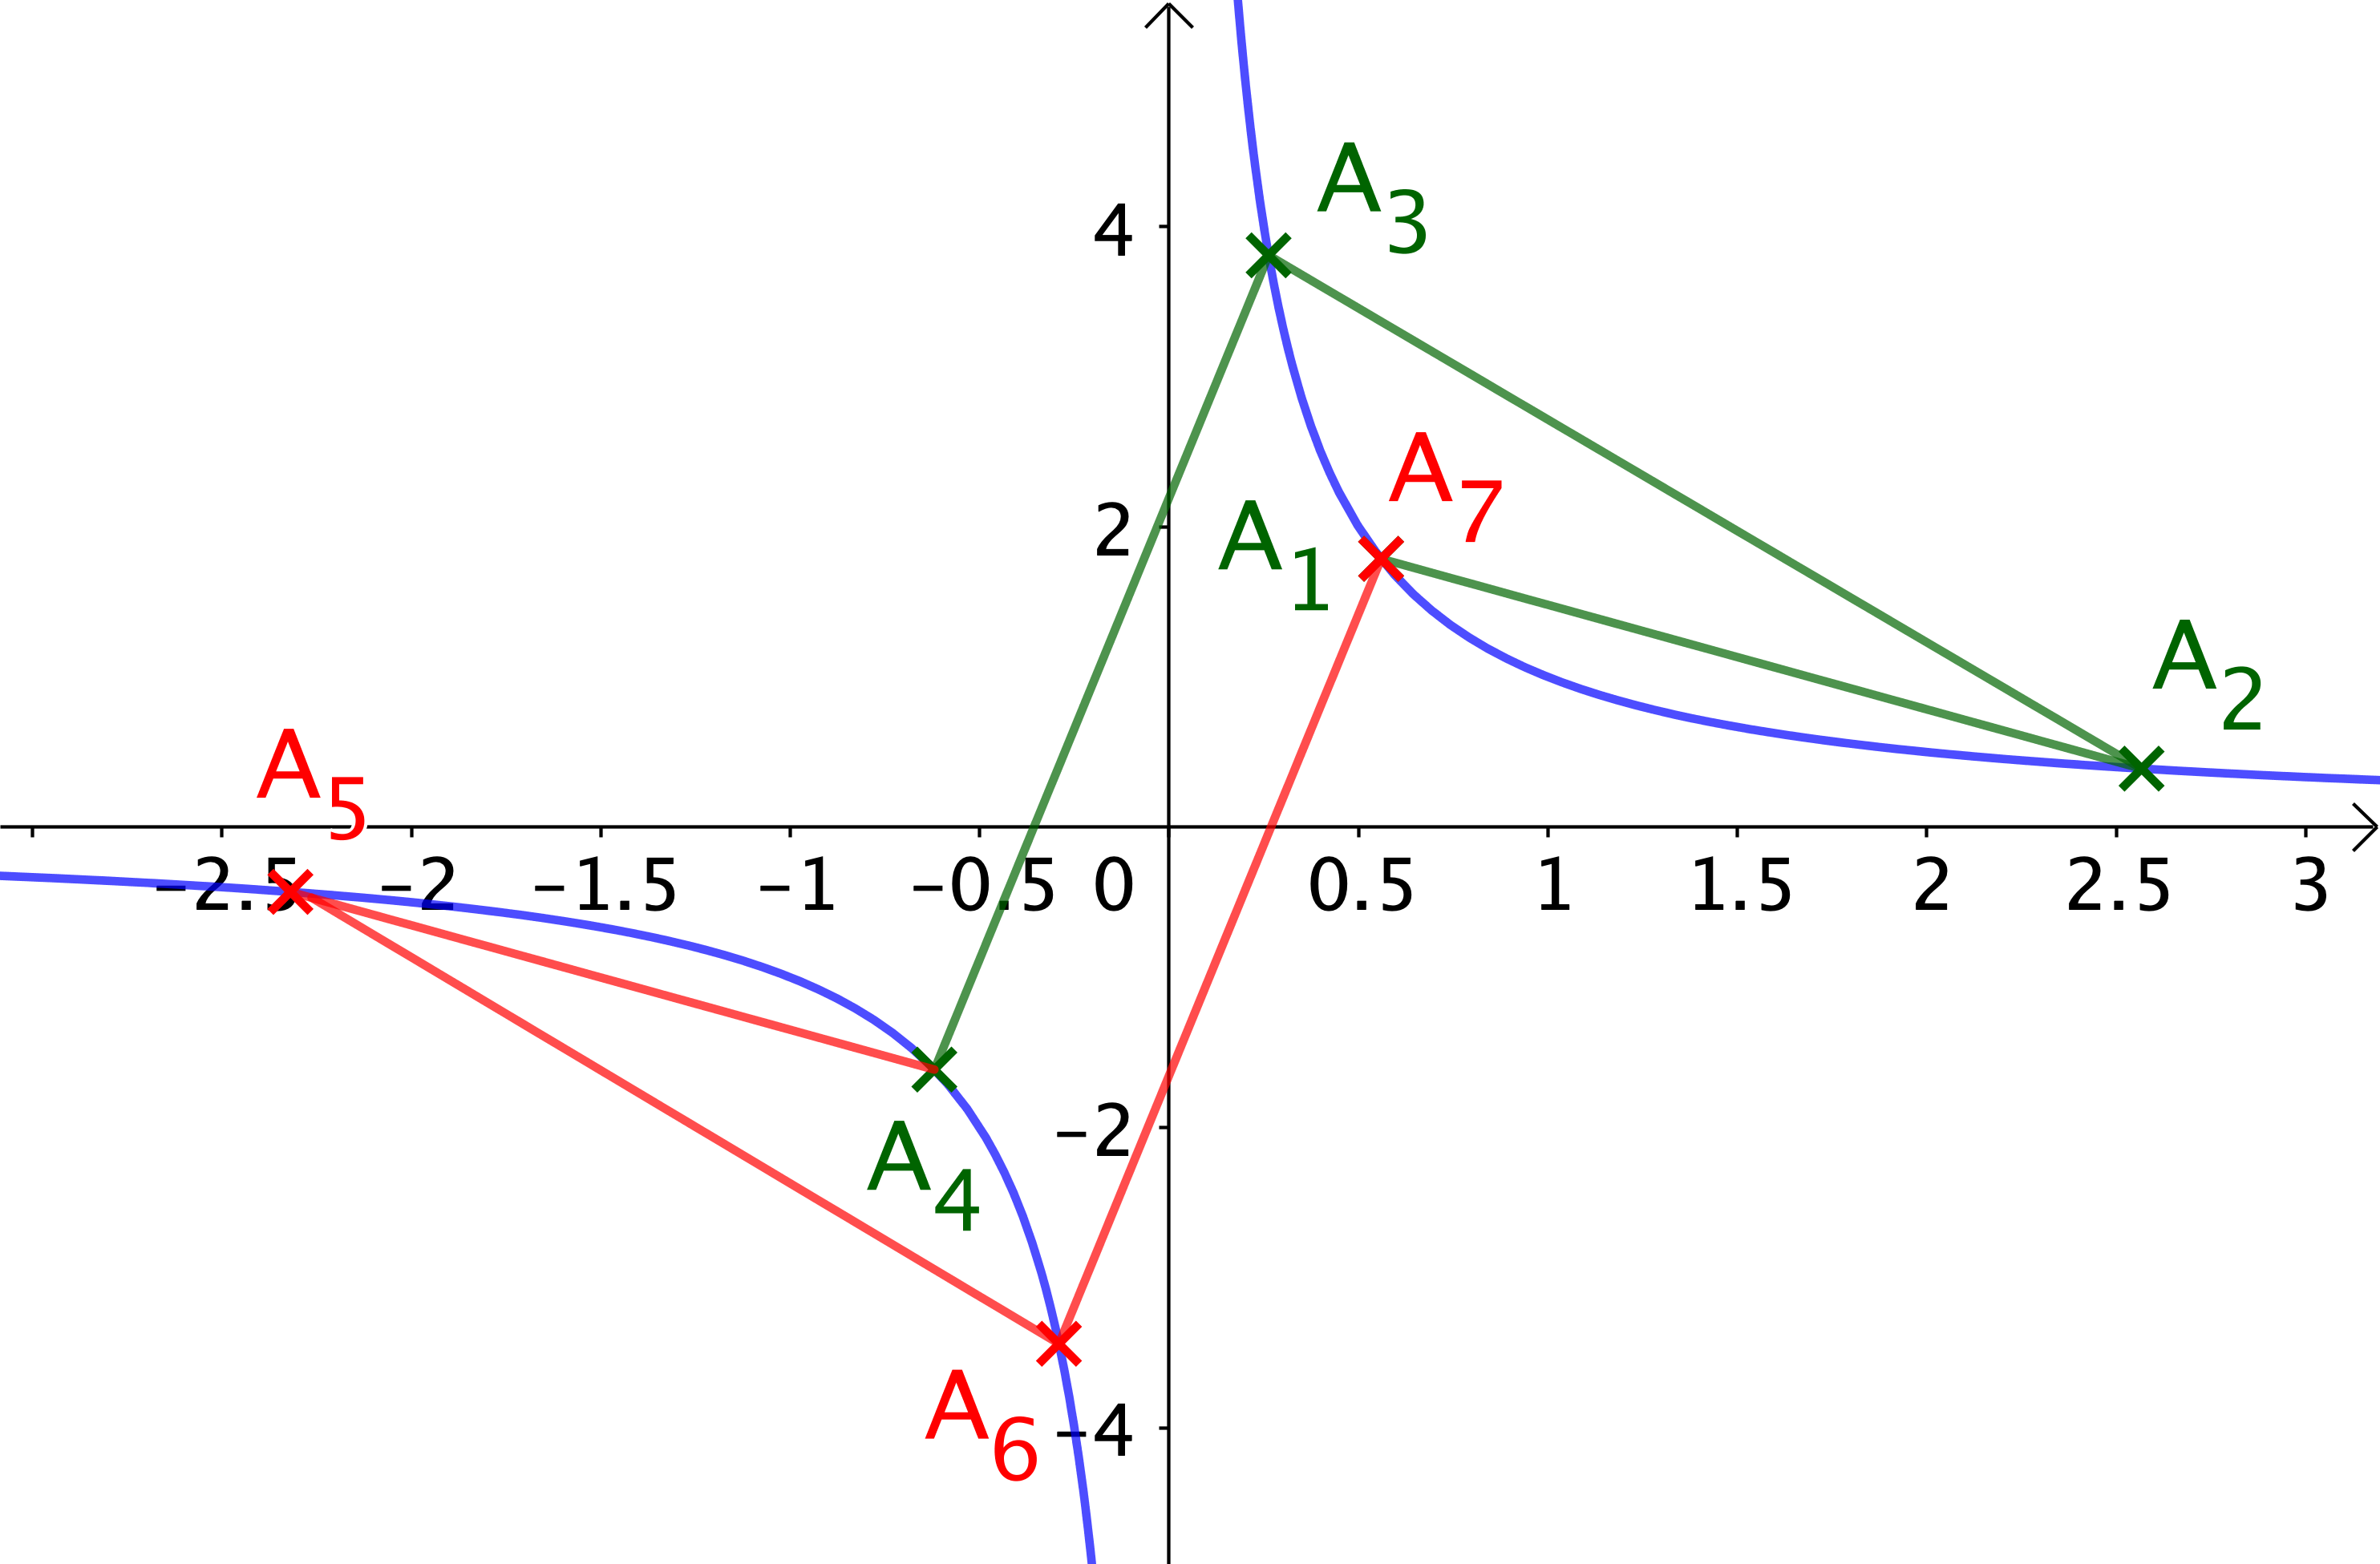
\includegraphics[scale = .8]{hyperbola/conjecture.png}}
\end{center}

\vspace{1em}

 
La preuve est similaire à celle faite pour la parabole
\footnote{
	Le lecteur habitué notera qu'ici la preuve est de nouveau algébrique car on utilise juste du calcul différentiel sur des fractions polynomiales à une variable.
}.
Ici la pente d'une corde généralisée $\setgeo*{C}{MN}$ est $\left( - \frac{1}{x_M y_N} \right)$ comme nous allons le vérifier.
\begin{enumerate}
	\item Si $M \neq N$ , $\setgeo*{C}{MN} \eq[def] (MN)$ a pour pente $\frac{y_M - y_N}{x_M - x_N} = \frac{1}{x_M - x_N} \left( \frac{1}{x_M} - \frac{1}{x_N} \right) = - \frac{1}{x_M y_N}$ .

	\item Si $M = N$ , $\setgeo*{C}{MN}$ est la tangente en $M$ à la parabole $\setgeo{P}$ . Cette tangente admet pour pente $- \frac{1}{x_M^2} = - \frac{1}{x_M y_N}$ .
\end{enumerate}


\medskip

Nous avons alors les égalités suivantes où de nouveau $x_i \eq[def] x_{(A_i)}$ , les équivalences venant du fait qu'aucun des $x_i$ n'est nul :
\begin{itemize}[label=\small\textbullet]
	\item \textbf{[L1]} : 
	      $- \frac{1}{x_1 y_2} = - \frac{1}{x_4 y_5}$
	      $\,\, \Longleftrightarrow \,\,$
	      \textbf{[M1]} : 
	      $x_1 x_{2} = x_{4} x_{5}$

	\item \textbf{[L2]} : 
	      $- \frac{1}{x_2 y_3} = - \frac{1}{x_5 y_6}$
	      $\,\, \Longleftrightarrow \,\,$
	      \textbf{[M2]} : 
	      $x_2 x_{3} = x_{5} x_{6}$

	\item \textbf{[L3]} : 
	      $- \frac{1}{x_3 y_4} = - \frac{1}{x_6 y_7}$
	      $\,\, \Longleftrightarrow \,\,$
	      \textbf{[M3]} : 
	      $x_3 x_{4} = x_{6} x_{7}$
\end{itemize}


\medskip

\textbf{[M3] $\div$ [M2] $\times$ [M1]}
\footnote{
	Le lecteur connaissant la théorie des groupes voit tout de suite que nous avons là une version multiplicative dans $(\RRs , \times)$ du système additif dans $(\RR , +)$ vu pour la parabole.
	Dès lors nul besoin d'expliquer de nouveau comment déduire  $x_1 = x_7$ du système.
}
nous donne $x_1 x_4 = x_7 x_4$ d'où $x_1 = x_7$ puis $A_7 = A_1$ .
La section qui suit va permettre, via la notion de groupe, de comprendre pourquoi la construction magique fonctionne sur un cercle, la parabole $\setgeo{P} : y = x^2$ et l'hyperbole $\setgeo{H} : y = \frac{1}{x}$ .
